\chapter{Implementierung} \label{implementation}

Dieses Kapitel erläutert den Implementierungsvorgang des Java Medical Imaging Toolkits. Besonderer Wert wird auf die Umsetzung der Blattknoten wie in Kapitel \ref{architecture} Abschnitt \ref{jmedikit_structure} gelegt, da diese Anwendungsteile direkt mit dem Anwender in Aktion treten.\\
Nach einer Beschreibung wie die DICOM-Objekte repräsentiert werden, wird umfangreich auf die Bilddarstellung und Manipulation eingegangen.

\section{Implementierung der DICOM-Objekte}

Die beiden Schnittstellen \textit{IDicomData} und \textit{IDicomImageData} bilden die Grundlagen aller DICOM-Objekte die vom jMediKit erzeugt werden und sind gleichzeitig die einzige Kommunikationsmöglichkeit zu den externen Bibliotheken. Der abstrakte Adapter \textit{ADicomObject} stellt die Funktionen beider Schnittstellen zur Verfügung. Die wichtigsten Methoden stellen das Auslesen der Pixel und den einzelnen Tags eines DICOM-Objekts dar. \\
Das eingebundene \textit{dcm4che} bietet neben der Verarbeitung von DICOM-Objekten auch eine Implementierung des Kommunikations- und Speicherstandards von DICOM an. Während der aktuellen Entwicklung wurde allerdings nur ein Bruchteil der DICOM-Verarbeitung zur Erfüllung der Anforderungen benötigt und der Kommunikations- und Speicherprozess fand keine Beachtung. Bei einer Implementierung sollte dennoch eine zukünftige Erweiterung im Auge behalten werden. Dabei soll ebenso das Open-Closed-Prinzip Beachtung finden.\\
Hierbei werden die Schnittstellen in fachspezifische Domänen eingeteilt. Das bedeutet \textit{IDicomData} ist für das Verarbeiten der Tags zuständig, während \textit{IDicomImageData} ausschließlich Bilddaten verarbeitet. Für weitere Versionen können weitere Domänen implementiert werden, wie zum Beispiel eine Schnittstelle \textit{IDicomNetworkData}. Der Adapter vereint die Domänen zu einem vollen DICOM-Objekt. 

\section{Der DicomBrowser}
Der DicomBrowser ist der zentrale Part zum Transfer der DICOM-Dateien aus dem Dateisystem zu les- und verarbeitbaren DICOM-Objekten. Abbildung \ref{dicombrowser} zeigt die Darstellung nach dem Einlesenen eines Ordners mit DICOM-Dateien. Die Repräsentation entspricht dem ER-Modell aus Kapitel \ref{grundlagen} Abschnitt \ref{grundlagen:iod}. Der Knoten $\backslash$ symbolisiert die Wurzel. \textit{BRAINX}\footnote{Beispieldatensätze verfremden die tätslchlichen Patientennamen. Originale Datensätze hätten die Form \textit{Nachname\^{}Vorname}} steht für den Patientenname, gefolgt von in diesem Beispiel einer Studie, die wiederum aus sieben Serien besteht. Die einzelnen DICOM-Objekte als Blattknoten werden aufgrund der Übersichtlichkeit nicht angezeigt.\\
Die Repräsentation der Dateien ist nicht immer geordnet wie es das ER-Modell vorgibt und man kann nicht von einer sortierten Ordnerstruktur ausgehen. Die PACS-Software \textit{dcm4chee} ordnet die Daten beispielsweise nach dem Aufnahmedatum. Es wird eine Datenstruktur benötigt, die der DICOM Object Definiton entspricht.

\begin{figure}[htbp]
  \vspace{0.5cm}
  \centering
  \fbox{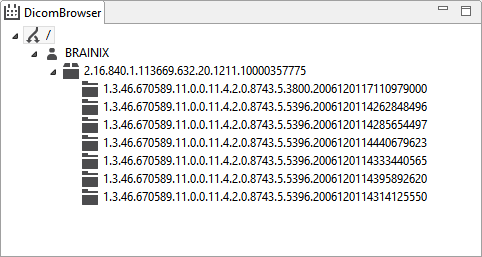
\includegraphics[angle=0,width=9cm]{./img/dicombrowser.png}}
   \caption{Die Baumansicht des DICOM-Browsers mit geladenen Objekten}
  \label{dicombrowser}
  \vspace{0.5cm}
\end{figure}

\subsection{Die Baumstruktur}
Sowohl die Anzeige, als auch die interne Behandlung der Daten soll so nah wie möglich an den DICOM-Standard angelehnt sein und soll unabhängig von der Auslieferung\footnote{Unabhängig davon, ob Dateien von der Festplatte geladen oder über das Netzwerk bezogen werden.} der Dateien die ER-Modell-Struktur haben. 

\subsection{Programmatische Erzeugung von DICOM-Objekten}

Das Java Medical Imaging Toolkit stellt zwei Möglichkeiten zur Verfügung Objekte in den Speicher einzulesen. So bietet die Klasse

\section{Repräsentation der Pixeldaten}

\section{Zeichnen der Bilddaten mit dem DicomCanvas}

\subsection{Implementierung der Werkzeuge}

\subsubsection{Das Bild bewegen mit dem MoveTool}

\subsubsection{Skalierung mit dem ResizeTool}

\subsubsection{Justierung der Fensterung mit dem WindowTool}

\subsubsection{Punktauswahl mit dem PointTool}

\section{Das Utility-Fenster}

\subsection{Debugging mit dem ConsoleView}

\subsection{DICOM-Objekte über DicomTagView ausgeben}

\section{Implementierung des Hauptmenüs und der Werkzeugleiste}

\subsection{Das Hauptmenü}

\subsection{Die Werkzeugleiste}



